\chapter{Fast graph kernel classifier based on optical random features }
\label{chapter:fast_algorithm}
\newtheorem{lemma}{Lemma} 
Graphlet kernel  is a good method to solve graph classification problem but as we have seen in chapter \ref{chapter:background}, it suffers from a high computational cost. In this chapter, we take inspiration from graph sampling and averaging to propose a family of fast graph kernels that generalizes the graphlet kernel paradigm. We show how random features can be incorporated within the new framework to get a faster and competitive algorithm in graph classification. Finally, we describe how Optical Processing Units (OPUs) can be used to eliminate some significant computational cost altogether.

\section{Proposed algorithm}
We recall from chapter \ref{chapter:background} that the computational cost of graphlet kernel is $C_{gk}= O(\tbinom{v}{k} N_k C_k)$. As an attempt to lower this cost, using graph sampling we can compute an empirical approximation of $k$-spectrum vector so the new that cost becomes $C_{gk + gs}= O(C_S s N_k C_k)$. What changed is that $\tbinom{v}{k}$ is replaced with $C_S s$, but the question is whether that is enough or not. We recall that the minimum number of samples $s \sim N_k$ required to ensure some certainty sharply increases as the graphlet size increase. It is clear then that the number of graph samples is not the only bottleneck here but also the cost to compute $\varphi_k^{match}$, denoted by $C_{\varphi_k^{match}}=O(N_k C_k)$.

So we propose to replace $\varphi^{match}_k$ with another user-defined function $\varphi:\phlet \mapsto\R^m$ and keep everything else as it is. We obtain a family of algorithms referred to as Graph Sampling and Averaging (GSA-$\varphi$), described in Alg. \ref{alg:GSA}.

\begin{algorithm}[H]\label{alg:GSA}
\DontPrintSemicolon
  \KwInput{2-Classes labelled graph dataset $\mathcal{X}=(\G_i,y_i)_{i=1,\ldots,n}$}
  \KwOutput{Trained model to classify graphs}
  \tools{Graph random sampler $S_k$, a function $\varphi$, linear classifier (ex. SVM) }\\
  \Hyp{k:graphlet size, $s$:\#graphlet samples per graph}\\
  %\KwData{Testing set $x$}
  %$\sum_{i=1}^{\infty} := 0$ \tcp*{this is a comment}
  %\tcc{}
  \Algo{\\}
  Random initialization of SVM weights\\
  \For{$\G_i$ in $\mathcal{X}$}{
  $\varphi_i=0$\\
  \For{$j=1:s$}{
  $F_{i,j}\gets S_k(\G_i)$\\
  $\varphi_i\gets \varphi_i +\frac{1}{s}\varphi(F_{i,j})$
  }
  }
  $\mathcal{D}_{\varphi}\gets (\varphi_i,Y_i)_{i=1,\ldots, n}$\\
  Train the linear classifier on the new vector-valued dataset $\mathcal{D}_{\varphi}$
\caption{Graph Sampling and Averaging (GSA-$\varphi$)}
\end{algorithm}

We note that within the new paradigm, the defined $\varphi$ does not necessarily respect the isomorphism between sampled subgraphs: if $\varphi(F) = \varphi(F')$ whenever $F \cong F'$, then we are in the framework of graphlet \emph{without} repetition, otherwise we are in the other case. As we will see, choosing a randomized $\varphi$ presents both theoretical and practical advantages, however it does not respect isomorphism. Nevertheless, it is possible to apply some preprocessing function $Q$ invariant by permutation before passing it to a randomized $\varphi$, and in this case isomorphism is respected without any condition on $\varphi$. An example of such function is $Q:\R^{k\times k}\mapsto \R^k, Q(F)=Sort(Eigenvalues(\mathbf{A}_F))$, that is, the sorted eigenvalues of the adjacency matrix.

\todoNK{A word on the generic computational cost of the method ? $O(C_S s C_\varphi)$, emphasizing that $C_\varphi$ is now the main focus in the rest (intuitively, trade off between computational cost and discriminative power)}

\section{Using random features framework in our algorithm}
After we presented the generic algorithm, now we combine it with random features kernels.
Let's assume that we have a psd and shift-invariant graph kernel, as a recap, we know it can be written in the form:
\begin{equation}
\label{eq:random_features_3}
\mathcal{K}(F,F')= \mathbb{E}_w \xi_w(F)\xi_w(F')
\end{equation}
which gives that by defining:
\begin{equation}
\varphi(F) = \frac{1}{\sqrt{m}} ( \xi_{w_j}(F) )_{j=1}^m \in \mathbb{C}^m,~~~ m\in \mathbb{N}
\end{equation}
we can write:
\[
\mathcal{K}(F,F')\approx \varphi(F)^*\varphi(F')
\]
In this point and based on such kernel, we define another one, called \emph{mean kernel} $\K_{mk}$, with presenting its corresponding metric, called \emph{Maximum Mean Discrepancy (MMD)}. Next, we show with the aid of concentration inequalities how using the random features map $\varphi$ of $\K$ in  our algorithm $GSA-\varphi$ will lead to an approximation of $\K_{mk}$ concentrated around its true value with high probability.

The mean kernel methodology allows to \emph{lift} a kernel from a domain $\phlet$ to a kernel on \emph{probability distributions} on $\phlet$. Given a base kernel $\K$ and two probability distribution $\mathcal{P},\mathcal{Q}$, it is defined as:
\begin{equation}
\label{eq:mean_kernel}
\mathcal{K}_{mk}(\mathcal{P},\mathcal{Q}) = \mathbb{E}_{x \sim \mathcal{P}, y \sim \mathcal{Q}} \mathcal{K}(x,y)
\end{equation}
In other words, the mean kernel is just the expectation of the base kernel with respect to each term. Mean kernel is associated to an Euclidean metric which is referred to with the  \emph{Maximum Mean Discrepancy (MMD)}, and is defined as:
\begin{equation}\label{eq:MMD}
MMD(\mathcal{P},\mathcal{Q}) = \sqrt{\mathcal{K}_{mk}(\mathcal{P},\mathcal{P}) + \mathcal{K}_{mk}(\mathcal{Q},\mathcal{Q}) - 2\mathcal{K}_{mk}(\mathcal{P},\mathcal{Q})}
\end{equation}
It should be noticed here that $\mathcal{K}_{mk}(\mathcal{P},\mathcal{P}) = \mathbb{E}_{x \sim \mathcal{P}, x' \sim \mathcal{P}} \mathcal{K}(x,x') \neq \mathbb{E}_{x \sim \mathcal{P}} \mathcal{K}(x,x)$.

\textbf{The link between the mean kernel and graphs} can be easily constructed, since considering a random sampling method $S_k$, the pair $(S_k , \G)$  introduces a probability distribution on the set of size-$k$ graphlets $\phlet$. Thus, for two graphs $\G,\G'$ , the mean kernel can be reformulated to:
\begin{equation}
\label{eq:mean_kernel_graphs}
\mathcal{K}_{mk}(\G,\G')= \mathbb{E}_{F \sim S_k(\G), F' \sim S_k(\G')} \mathcal{K}(F,F')
\end{equation}
A special case is to  consider the uniform sampler, which satisfies $Pr(S_k(\G)=\phlet_i)=(f_\G)_i$, where the mean kernel is reduced to:
\[
\mathcal{K}_{mk}(f_\G,f_\G')=\sum_{i,j}^{N_k}(f_\G)_i(f_{\G'})_j\mathcal{K}(\phlet_i,\phlet_j) 
\]

Now to integrate random features with the mean kernel, we combine the decomposition of the base kernel $\mathcal{K}$ in Eq. \ref{eq:random_features_3} with Eq.\ref{eq:mean_kernel_graphs} to get:
\begin{equation}
    \label{eq:mk_rf}
    \mathcal{K}_{mk}(\G,\G')= \mathbb{E}_{F \sim S_k(\G), F' \sim S_k(\G')} \mathbb{E}_w \xi_w(F)\xi_w(F')
\end{equation}
The corresponding MMD metric in this case is:
\begin{equation}
\label{eq:MMD-RF}
MMD(\G,\G')^2 = \mathbb{E}_{\omega} \Big( | \mathbb{E}_{S_k(\G)} \xi_\omega(F) - \mathbb{E}_{S_k(\G')} \
\xi_\omega(F') |^2 \Big)
\end{equation}

Until now, what we have in Eq. \ref{eq:mk_rf} is the true value of the mean kernel, where the expectations there implies that we should consider infinite number of both graph samples and random features. However, what we really want is to approximate this value using our algorithm $GSA-\varphi$, which includes  using the  map $\varphi$ of $\mathcal{K}$ and a finite number of \emph{iid} samples with $S_k$. First let's consider only a finite number $s$ of samples: $\F_\G=\{F_1, \ldots, F_s\}$ and $\F_{\G'}=\{F'_1, \ldots, F'_s\}$. Then we have: 
\begin{equation}
\label{eq:MK_samples}
\mathcal{K}_{mk}(\G,\G') \approx \frac{1}{s^2} \sum_{i,j=1}^s \mathbb{E}_w \xi_w(F_i)\xi_w(F'_j)
\end{equation}
\[
MMD(\G,\G')^2 \approx \frac{1}{s^2}\mathbb{E}_{\omega} ( | \xi_\omega(F) -\xi_\omega(F') |^2 )
\]
No we advance another step and consider a finite number $s$ of \emph(iid) samples and a feature map $\varphi$ with finite number $m$ of random features, so the formula of our final approximation is:
\begin{equation}
\label{eq:mean_kernel_RF}
\mathcal{K}_{mk}(\G,\G') \approx \frac{1}{s^2} \sum_{i,j=1}^s \varphi(F_i)^*\varphi(F_j')=\Big(\frac{1}{s}\sum_{i=1}^s\varphi(F_i)\Big)^*~\Big(\frac{1}{s}\sum_{i=1}^s\varphi(F_i')\Big)
\end{equation}
\[
MMD(\G,\G')^2 \approx  \| \frac{1}{s}\sum_{i=1}^s\varphi(F_i) -\frac{1}{s}\sum_{i=1}^s\varphi(F_i') \|_2^2 
\]

Indeed, we just proved that based on the assumption on the base kernel $\mathcal{K}$ in Eq. \ref{eq:random_features_3}, $GSA-\varphi$ theoretically represents an unbiased estimation of the mean kernal $\mathcal{K}_{mk}$. Now, we have two issues to discuss: how is this estimation concentrated around its expected value $\mathcal{K}_{mk}$, and what is the computational cost of $GSA-\varphi$ in this case. While the first question can be addressed for any kernel $\mathcal{K}$, the second one is really case-dependent as it is mainly related to the computational cost of computing the term $\varphi(F_i)$ in Eq. \ref{eq:mean_kernel_RF} which differs from one $\mathcal{K}$ to another. We start answering the first question.


\begin{theorem}
\label{theorem:concentration}
Let $\G$ and $\G'$ be two graphs, $\{F_i\}_{i=1}^{s}$ (resp. $\{F_i'\}_{i=1}^{s}$) be $iid$ size-k graphlet samples drawn from $\G$ (resp. $\G'$). We have that $\forall \epsilon >0$:
\begin{align*}
    Pr\Big(\Big | \mathcal{K}_{mk}(\G,\G') - \| \frac{1}{s} \sum_i \varphi(F_i) - \frac{1}{s} \sum_i \varphi(F'_i)\|\Big | \geq
    \epsilon\Big)\leq e^{-\frac{(\epsilon\sqrt{s}-2)^2}{4}}
\end{align*}
\end{theorem}
this tells that the estimation converges to its expected value exponentially in $\sqrt{s}$, which is a good support to the proposed algorithm. However the proof of this theorem is provided in section \ref{section:proof}.

To calculate \textbf{the computational cost of $GSA-\varphi$}, we considered three cases of $\varphi$, hence $\mathcal{K}$, in both theoretical and practical sides: Gaussian random features applied on the adjacency matrix, Gaussian random features applied on the Eigenvalues of the adjacency matrix , and finally the optical random features of OPUs. The case of OPU random features is presented in section \ref{section:OPU}.\newline
For a flattened version of an adjacency matrix $\mathbf{A}_{flat}$ of a subgraph $F$, we recall that the Gaussian kernel stated in Eq. \ref{eq:Guassian_kernel} can be approximated by the inner product of the following random features map:
\[
\varphi(\mathbf{A}_{flat}) = \frac{1}{\sqrt{m}} ( \sqrt{2}cos(w_j^T\mathbf{A}_{flat}+b) )_{j=1}^m \in \mathbb{C}^m
\]
where $w_j\in\R^{k^2}$ drawn from the Gaussian distribution in Eq. \ref{eq:G_fourier}. Hence, The computational cost needed in this case for each subgraph to compute its $\varphi(\mathbf{A}_{flat})$ is $O(mk^2)$ . Which is the cost of matrix multiplication supposing that we have a fast method to evaluate the $cos$ function. Finally, the processing cost per graph $\G$ is: $C_{Gs}=O(smk^2)$.

Gaussian random features applied on the Eigenvalues of the adjacency matrix is similar to the one applied on the adjacency matrix, the difference is that instead of passing the adjacency matrix as an input, we pass a vector of its Eigenvalue $\boldsymbol{\lambda}\in\R^k$. So what changes per subgraph process is the input dimension and the cost of Eigenvalues extraction, which is $O(k^3)$. In a similar way, we can write: $C_{Gs+Eig}=O(s(mk+k^3))$.



\section{Fast $GSA-\varphi$ with optical random features}
\label{section:OPU}
Optical processing units (OPUs) are physical units developed to apply optical random features projections in light-speed. In this section and before introducing $GSA-\varphi$ in its ultimate and fastest form $GSA-\varphi_{OPU}$, we explain what optical random features projection is. We start by presenting the mathematical model of these projections $\varphi_{OPU}$, next we explain how OPUs can perform such projections in light-speed from hardware point of view. Finally, we merge OPUs' random features with our proposed algorithm and compare the corresponding computational cost with previously mentioned methods.

\subsection{Optical random features model}
Random projections is one of the important techniques in machine learning and in signal processing. However, traditional random projection methods need a large memory to store the corresponding random matrix $\mathbf{W}$ and a huge computational time to project the input data points $\mathbf{x}$, i.e. to compute $\mathbf{Wx}$. Optical processing units (OPU's) is the technology developed to solve the previous two drawbacks: where an OPU complete random projections at the speed of light without the need to store any random matrix. In general, Random projections are the result of two procedures: the first one is the linear-random projections and the second one is non-linear mapping.
Mathematically speaking, OPU's perform the following operation \citep{saade_opu}:
\begin{equation}
\label{OPU_equation}
\mathbf{\varphi}_{OPU}(\mathbf{x})=|\mathbf{Wx+b}|^2 ;~\mathbf{W}\in \mathbb{R}^{m\times d},\mathbf{b}\in \mathbb{R}^m, \mathbf{x}\in \mathbb{R}^d
\end{equation}
Where $\mathbf{b}$ is a bias vector, $\mathbf{x}$ is an input point, $m$ is the number of random features, $d$ is the input space dimension and the amplitude function $|.|$ is taken element wise in $\mathbf{\varphi}_{OPU}(\mathbf{x})$. The matrix $\mathbf{W}$ is a random \emph{iid} complex matrix with Gaussian real and imaginary parts.\newline
In the limit where the number of random features $m\xrightarrow{}\infty$, it can be proven by the concentration of the measure that the inner product between the projected data points $(\mathbf{\varphi}_{OPU}(\mathbf{x}\in \mathbb{R}^m)$ in the new feature space tends to a kernel function that depends only on the input points in the original feature space $(\mathbf{x}\in \mathbb{R}^d)$

\subsection{OPU structure and functionality}
Eq.~\ref{OPU_equation} still imply that an OPU need to store and multiply by the random projection matrix. But in an OPU, a heterogeneous material, as a paper or any white translucid material, is used to scatter incident light in a very complex way. The behavior of the scattering process is considered random because of the extremely high complexity. One can argue that light scattering is a linear, deterministic, and reproducible phenomenon, but what can be said here is that the unpredictable behavior of the process makes it effectively a random process. That is why these materials are called opaque since all information embedded within the incident light is seemingly lost during the propagation through the material \citep{saade_opu}. An example used to demonstrate and justify the resulted randomness is a cube of edge length $100\mu m$, such cube can include $\approx 10^7$ paint nanoparticles, all the positions and shape of these particles must be known in order to predict its effect on light. Propagation through such a layer can be seen as a random walk because of frequent scattering with the nanoparticles, where light explores the whole volume and undergoes tens of thousands of such scattering steps before coming out from the other side in a few picoseconds.\newline

\begin{figure}[ht!]
\begin{center}
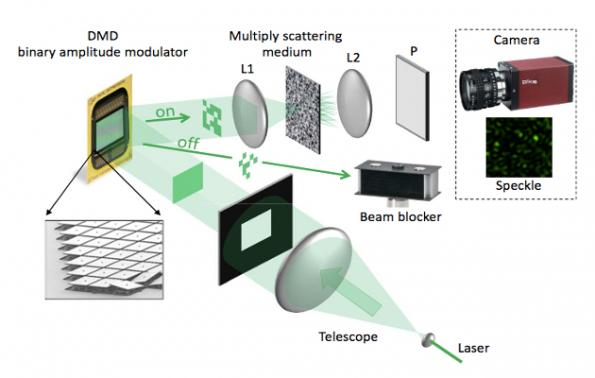
\includegraphics[scale=0.5]{figs/lighton630.jpg}
\end{center}
\caption[OPU's Experimental setup]{OPU's Experimental setup \citep{saade_opu}: A monochromatic laser is expanded by a telescope, then
illuminates a digital micromirror device (DMD), able to spatially encode digital information on the light beam by
amplitude modulation. The light beam carrying the signal is then focused on a random
medium by means of a lens. The transmitted light is collected on the
far side by a second lens, passes through a polarizer, and is measured by a standard monochrome CCD camera for example .}
\label{fig_opu}
\end{figure}
When the incident light is coherent, it promotes complex interference patterns, called speckles, due to the scattering process.
These speckles don't only characterize the propagation medium but also the incident light, and this can be modeled by $y=Wx$, 
where $y$ and $x$ are the vector amplitudes between a set of spatial modes at the output and at the input of the medium respectively. In OPUs, the transmission matrix $W$ of the propagation medium can be approximately considered as a Gaussian i.i.d matrix, it was also shown that even without $W$ being known, but it is guaranteed to be stable as long as the propagation medium is stable as a paint layer for instance \citep{saade_opu}.  So if we use a spatial light modulator and a laser to send an appropriate set of illuminations to the propagation medium, we can acquire the output intensity $|y|^2$ with a CCD or CMOS camera, and that is the principle concept behind OPU's functionality as seen in Fig~ \ref{fig_opu}.\newline 
The DMD (digital micromirror device) used in OPU's is a binary amplitude modulator consisting of an array of micro-mirrors, Each mirror can be lit or not, thus it can represent  a binary value. In order to represent grey values, each value is encoded on a square sub-array ($4\times 4$ for example) in the DMD, where the number of lit mirrors reflects the desired level of grey. DMD reflects the data and send the reflected light through the disordered medium, then a snapshot of the resulting random projection is acquired using a standard camera. all that is completed in a very high speed compared to the traditional random features techniques. 
\subsection{Fast $GSA-\varphi_{OPU}$ algorithm with complexity discussion}
After what we presented about OPUs and optical random features projections, we can efficiently deploy $\varphi_{OPU}$ random feature map in $GSA-\varphi$ framework. The resulted pseudo code is presented below and we refer to the resulted algorithm with $GSA-\varphi_{OPU}$. \newline\newline
\begin{algorithm}[H]
\DontPrintSemicolon
  \KwInput{2-Classes labelled graph dataset $\mathcal{X}=(\G_i,y_i)_{i=1,\ldots,n}$}
  \KwOutput{Trained model to classify graphs}
  \tools{Graph random sampler $S_k$, optical processing unit (OPU), linear classifier (ex. SVM) }\\
  \Hyp{k:graphlet size, $s$:\#graphlet samples per graph}\\
  %\KwData{Testing set $x$}
  %$\sum_{i=1}^{\infty} := 0$ \tcp*{this is a comment}
  %\tcc{}
  \Algo{\\}
  Random initialization of the classifier weights\\
  \For{$\G_i$ in $\mathcal{X}$}{
  $\boldsymbol{\varphi}_{OPU}(i)=0$\\
  \For{$j=1:s$}{
  $F_{i,j}\gets S_k(\G_i)$\\
  $\mathbf{A}\gets adjacency\_matrix(F_{i,j})$\\
  $\boldsymbol{\varphi}_{OPU}(i)\gets \boldsymbol{\varphi}_{OPU}(i) +\frac{1}{s}\boldsymbol{\varphi}_{OPU}(F_{i,j})$
  }
  }
  $\mathcal{D}_{\varphi_{OPU}}\gets (\boldsymbol{\varphi}_{OPU}(i),y_i)_{i=1,\ldots, n}$\\
  Train the linear classifier on the new vector-valued dataset $\mathcal{D}_{\varphi_{OPU}}$
\caption{GSA-$\varphi_{OPU}$}
\end{algorithm}

\textbf{The computational cost} of this innovative version $GSA-\varphi_{OPU}$, and more specifically of computing $\boldsymbol{\varphi}_{OPU}(\mathbf{A})$, is $O(1)$ in both the number of random features and the graphlet size. One can reasonably argue that an OPU has its limits, as the DMD mirror array ,where the input $\mathbf{A}$ is encrypted, has a limited dimensions \emph(width $\times$ length). Moreover, the camera used to acquire the light intensity in an OPU has a limited number of pixels thus it introduces a limit on the maximum number of random features. However, our argument is that when we respect these limits, which are usually large ones, the computational cost is a constant in both $m$ and $k$. To better illustrate the advantage of $GSA-\varphi_{OPU}$ over other discussed methods in this work, we show a comparison between them with respect to the computational time per graph $\G$:
\begin{itemize}
    \item Graphlet kernel: $C_{gk}= O(\tbinom{v}{k} N_k C_k)$
    \item Graphlet kernel with sampling: $ C_{gk + gs}= O(C_s s N_k C_k)$
    \item Gaussian features $GSA_{\varphi_{Gs}}$: $C_{Gs}=O(smk^2)$
    \item Gaussian features  $GSA_{\varphi_{Gs}}$ with Eigenvalue preprocessing: $C_{Gs+Eig}=O(s(mk+k^3))$
    \item $GSA_{\varphi_{OPU}}$:  $C_{OPU}=O(1)$
\end{itemize}

\section{$GSA-\varphi$ concentration inequality proof}
\label{section:proof}

\begin{proof}
Here, we prove theorem \ref{theorem:concentration}, where We decompose the proof in two steps.
we first assume that:
\begin{equation}
\label{eq:z_assumption}
    0\leq z_\omega(F)\leq 1, \forall \omega \sim  \Lambda
\end{equation}
This is a reasonable assumption from what we have seen in random Fourier features maps referred to in Eq. \ref{eq:Fourier_xi}.
\paragraph{Step 1: infinite $s$, finite $m$ (number of random features).} Based on our assumption on $z_\omega$ in \eqref{eq:z_assumption}, it is a straight forward result of Hoeffding's inequality that  $d(G, G')^2$ is close to $\frac{1}{m} \sum_{j=1} | \mathbb{E}_{F \sim f_G} z_{\omega_j}(F) - \mathbb{E}_{F' \sim f_{G'}} z_{\omega_j}(F') |^2 = \| \mathbb{E}_{F \sim f_G} z(F) - \mathbb{E}_{F' \sim f_{G'}} z(F')\|^2$.  
\begin{lemma}[Hoeffding's inequality] 
Let $(x_1,\ldots, x_m)$ be independent random variables such that the variable $x_i$ is strictly bounded by the interval $[a_i , b_i]$, and let $\overline{X}=\frac{1}{m}\Sigma_{i=1}^{m}x_i$ then we have:
\begin{equation}
\label{eq:Hoeffding}
    Pr(|\mathbb{E}\overline{X}-\overline{X}|\geq \epsilon)\leq 2~ exp (-\frac{2m^2\epsilon^2}{\Sigma_{i=1}^m(b_i-a_i)^2)})
\end{equation}

\end{lemma}
%\begin
In our case, and for a finite number of random features $(m)$ we have the variables $x_j=| \mathbb{E}_{F \sim f_G} z_{\omega_j}(F) - \mathbb{E}_{F' \sim f_{G'}} z_{\omega_j}(F') |^2 $ are independent and bounded by the interval $[0,1]$ too, thus it is an easy result to see that:
\begin{equation}
    Pr(\Big|\frac{1}{m} \sum_{j=1}^m | \mathbb{E}_{F \sim f_G} z_{\omega_j}(F) - \mathbb{E}_{F' \sim f_{G'}} z_{\omega_j}(F') |^2 - \mathbb{E}_{\omega}  | \mathbb{E}_P z_\omega(x) - \mathbb{E}_Q z_\omega(x) |^2 \Big| \geq \epsilon) \leq 2~ e^{ -2m\epsilon^2}
\end{equation}

\paragraph{Step 2: finite ${s}$ and $m$.} We show that for any \emph{fixed} set of random features $\omega_j$, we have $\| \mathbb{E}_{F \sim f_G} z(F) - \mathbb{E}_{F' \sim f_{G'}} z(F')\|$ close to $\| \frac{1}{{s}} \sum_i z(F_i) - \frac{1}{{s}} \sum_i z(F'_i)\|$.  \newline
Let us consider a fixed set of random variables $\{\omega_j\}_{j \in \{1,\ldots, m\}}$ drawn independently from $\Lambda$, thus the random features map of a graph F equals: $z(F) = \frac{1}{\sqrt{m}}\left[z_{\omega_j}(F)\right]_{j=1}^m$.\newline
For every graph G , let $F_1,\ldots, F_{s}$ be ${s}$ random subgraphs drawn independently from G, we clearly have: 
\begin{equation}
\label{eq:subsample}
    \mathbb{E}_{F \sim f_G} z(F)= \mathbb{E} (~\frac{1}{{s}} \sum_i z(F_i)~)
\end{equation} 
What should be noticed now to be used later is that $\forall F\sim f_G, z(F)$ is in a ball $\mathcal{H}$ of radius $M=\frac{\sqrt{m}}{\sqrt{m}}=1$.
\begin{lemma}
\label{lemma:vector_hoeffding}
let $X=\{x_1,\ldots,x_{s}\}$ be $iid$ random variables in a ball $\mathcal{H}$ of radius $M$ centered around the origin in a Hilbert space. Denote their average by $\overline{X}=\frac{1}{{s}}\sum_{i=1}^{s}x_i$. Then for any $\delta>0$, with probability at lest $1-\delta$, 
\begin{equation}
\label{eq:vector_hoeffding0}
  \| \overline{X}-\mathbb{E}\overline{X}\|\leq \frac{M}{\sqrt{{s}}}(1+\sqrt{2~log\frac{1}{\delta}}
\end{equation}
\end{lemma}
\begin{proof}
Defining the function $f(x)= \| \overline{X}-\mathbb{E}\overline{X}\|$, and $\widetilde{X}={x_1,\ldots,\widetilde{x}_i,\ldots,x_{s}}$ to be a copy of $X$ with the ith element replaced by an arbitrary element of $\mathcal{H}$, we can prove using the triangle inequality:
\begin{equation}
    |f(X)-f(\widetilde{X})|=\Big|\| \overline{X}-\mathbb{E}\overline{X} \|-\|\overline{\widetilde{X}} - \mathbb{E}\overline{X}  \| \Big|\leq \| \overline{X} - \overline{\widetilde{X}}\|\leq
    \frac{\|x_i - \widetilde{x_i} \|}{{s}}\leq
    \frac{2M}{{s}}
\end{equation}
Therefor, $f(X)$ is insensitive to the ith component of $X,~ \forall i \in \{1,\ldots,{s}\}$ which is an important requirement to apply McDiarmid's inequality on $f$. \newline
To bound the expectation of $f$, we use the familiar identity about the variance of the average of $iid$ random variables:
\begin{equation}
\mathbb{E}\|\overline{X}-\mathbb{E}\overline{X}\|^2=\frac{1}{n}(\mathbb{E}\|x\|^2-\|\mathbb{E}x\|^2 ) 
\end{equation}
Also:
\[ \mathbb{E}f(X)\leq\sqrt{\mathbb{E}f^2(X)}=\sqrt{\mathbb{E}\|\overline{X}-\mathbb{E}\overline{X}\|^2}\leq \frac{M}{\sqrt{{s}}}\]
This bound for the expectation of $f$ and McDiamid's inequality give: 
\begin{equation}
\label{eq:vector_hoeffding1}
    Pr_x \Big [ f(X)-\frac{M}{\sqrt{{s}}}\geq \epsilon \Big ]\leq
    Pr_x \Big [ f(X)-\mathbb{E}f(X)\geq \epsilon \Big ]\leq
    exp\Big( -\frac{{s}\epsilon^2}{2M^2}\Big)
\end{equation}
Which is equivalent to \eqref{eq:vector_hoeffding0} by setting $\delta=exp( -\frac{{s}\epsilon^2}{2M^2})$ and solving for $\epsilon$.
\end{proof}
Now back to Eq. \eqref{eq:subsample} and its corresponding assumptions that we made, we can directly apply lemma \ref{lemma:vector_hoeffding} (and more especially Eq.\eqref{eq:vector_hoeffding1}) to get that:
\begin{equation}
    \label{eq:fixed_w}
    Pr(\|\mathbb{E}_{F \sim f_G} z(F)-~\frac{1}{n} \sum_i z(F_i)~\|\geq \frac{1}{\sqrt{n}}+\epsilon)\leq
    e^{-\frac{n\epsilon^2}{2}}
\end{equation}
Now applying the triangle inequality again yields:
\begin{align*}
    \Big | \| \mathbb{E}_{F \sim f_G} z(F) - \mathbb{E}_{F' \sim f_{G'}} z(F')\| - \| \frac{1}{{s}} \sum_i z(F_i) - \frac{1}{{s}} \sum_i z(F'_i)\|\Big | \leq  \\
   \| (\mathbb{E}_{F \sim f_G} z(F) -  \frac{1}{{s}} \sum_i z(F_i) )- (\mathbb{E}_{F' \sim f_{G'}} z(F') - \frac{1}{{s}} \sum_i z(F'_i))\|\leq \\
    \| \mathbb{E}_{F \sim f_G} z(F) -  \frac{1}{{s}} \sum_i z(F_i) \|+ \|\mathbb{E}_{F' \sim f_{G'}} z(F') - \frac{1}{{s}} \sum_i z(F'_i)\|
\end{align*}
Thus, since the two variables $\| \mathbb{E}_{F \sim f_G} z(F) -  \frac{1}{{s}} \sum_i z(F_i) \|$ and $\|\mathbb{E}_{F' \sim f_{G'}} z(F') - \frac{1}{{s}} \sum_i z(F'_i)\|$ are independent (as a direct result of our aforementioned assumption of independent random sampling), $\forall \epsilon>0$ we have:
\begin{align*}
    Pr( \| \mathbb{E}_{F \sim f_G} z(F) -  \frac{1}{{s}} \sum_i z(F_i) \| \geq \frac{1}{\sqrt{{s}}}+\frac{\epsilon}{2}, \|\mathbb{E}_{F' \sim f_{G'}} z(F') - \frac{1}{{s}} \sum_i z(F'_i)\|\geq\frac{1}{\sqrt{{s}}}+\frac{\epsilon}{2})=\\
    Pr( \| \mathbb{E}_{F \sim f_G} z(F) -  \frac{1}{{s}} \sum_i z(F_i) \| \geq \frac{1}{\sqrt{{s}}}+\frac{\epsilon}{2})~Pr( \|\mathbb{E}_{F' \sim f_{G'}} z(F') - \frac{1}{{s}} \sum_i z(F'_i)\|\geq\frac{1}{\sqrt{{s}}}+\frac{\epsilon}{2})\leq 
    e^{-\frac{{s}\epsilon^2}{4}}
\end{align*}
finally, we get as a straight result from above:
\begin{align*}
    Pr(\Big | \| \mathbb{E}_{F \sim f_G} z(F) - \mathbb{E}_{F' \sim f_{G'}} z(F')\| - \| \frac{1}{{s}} \sum_i z(F_i) - \frac{1}{{s}} \sum_i z(F'_i)\|\Big | \geq
    \frac{2}{\sqrt{{s}}}+\epsilon)\leq e^{-\frac{n\epsilon^2}{4}}
\end{align*}
And that is true for any fixed set of random variables  $\{\omega_j\}_{j \in \{1,\ldots, m\}}$ drawn independently from $\Lambda$.
Since it is valid for any fixed set of random features, it is also valid with \emph{joint} probability on random features and samples, by the \emph{law of total probability}. So we can write:
\begin{align*}
    Pr(\Big | \mathbb{E}_{\omega} \Big( | \mathbb{E}_{f_G} z_\omega(F) - \mathbb{E}_{f_{G'}} z_\omega(F') |^2 \Big) - \| \frac{1}{s} \sum_i z(F_i) - \frac{1}{s} \sum_i z(F'_i)\|\Big | \geq
    \frac{2}{\sqrt{s}}+\epsilon)\leq e^{-\frac{s\epsilon^2}{4}}
\end{align*}

\end{proof}


